
Elementary particles are affected by only four fundamental forces (or `interactions').  Gravity and the electromagnetic interaction are already familiar forces from our everyday experience, and in addition there are two nuclear forces, the strong interaction and the weak interaction.

\begin{table}
  \centering
  \fontfamily{ppl}\small\selectfont
  \begin{tabular}{lcc}
    \toprule
    Interaction & Range / m & Relative strength\\
    \midrule
    Strong & $\sim 10^{-15}$ & 1\\
    Electromagnetism & $\infty$ & $10^{-2}$\\
    Weak & $\sim 10^{-18}$ & $\sim 10^{-7}$\\
    Gravity & $\infty$ & $\sim 10^{-39}$\\
    \bottomrule
  \end{tabular}
  \caption{Summary of all four fundamental interactions.}
\end{table}

\subsection{Gravity}
Gravity affects all particles which have mass.  It has an infinite range and is purely attractive.  It governs the structure of stars, galaxies \&{}c.\ and its exact strength will determine the fate of the universe.

\subsection{Electromagnetism}
This interaction affects all particles with charge.  It is much stronger than gravity and also of infinite range, but it tends to cancel in bulk matter as this normally comprises nearly exactly equal numbers of positively and negatively charged particles.

\subsection{Strong}

The strong interaction is only felt by hadrons, which are all made from quarks.  The strong interaction is short range, and only affects nearest neighbours in the nucleus, as its range is the same as the diameter of a nucleon.  The strong interaction is always attractive, and charge independent (the same for n--p, p--p and n--n).

\begin{figure}
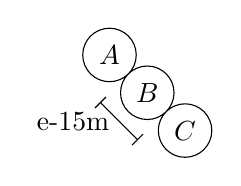
\begin{tikzpicture}[scale=1.2]
\draw (-0.4,0.4) node {$A$} circle (0.283) (0,0) node {$B$} circle (0.283) (0.4,-0.4) node {$C$} circle (0.283);
\draw[|-|] (-0.3,-0.3) node[anchor=east] {\SI{e-15}{m}} ++(-0.2,0.2)--++(0.4,-0.4);
\end{tikzpicture}
\caption{The strong interaction only affects nearest neighbours, i.e.\ $A$ and $B$ are attracted by the strong interaction, as are $B$ and $C$, but $A$ and $C$ are not.}
\end{figure}

\subsection{Weak}

When a neutron decays into a proton and an electron, an antineutrino is formed.  This is uncharged and does not feel the strong interaction, so another short range interaction must be involved.  The weak interaction affects both hadrons and leptons, and is usually associated with decays of various particles.  Weak decays generally take place much more slowly than strong decays (the stronger the interaction, the quicker the decay).

When \emph{strange} particles decay, they do so by the weak interaction, and strangeness is not conserved.

\subsection{Modern explanation of the four interactions}

It was previously thought that a particle creates a field which exists throughout all space, and this field affects any particles in the field, causing them to experience forces.  The modern view, however, is that two particles exert a force on one another due to the transfer of a virtual particle, which carries the interaction (this is known as second quantization).  These particles are called exchange particles, and are gauge bosons.

The amount of energy `borrowed' to create the mass/energy of the exchange particle\footnote{The energy to create these particles is `borrowed' according to the Heisenberg uncertainty principle, which allows energy $\Delta E$ to be created for a time $\Delta t$, so long as
\[\Delta E \times \Delta t < \hbar,\]
where $\hbar=\dfrac{h}{2\pi}=\SI{1.05e-34}{J.s}$, known as the reduced Planck constant.  Since the product of the energy and the time has to be below a certain limit, more massive exchange particles cannot exist for a long time, putting a limit on how far they may travel, and thus the range of the interaction.
} puts an upper limit on the range of the interactions produced.  This suggests:
\begin{itemize}
\item The range of electromagnetic and gravitational interactions is infinite, so the exchange particles for these interactions must be massless.
\item The range of the strong and weak are finite, so the exchange particles have mass, and the mass of the weak exchange particle is larger.
\end{itemize}

\subsection{The strong interaction}

Protons and neutrons are held together by the strong interaction (which acts on all hadrons).  As the range of the strong interaction is \SI{e-15}{m}, and assuming the exchange particle has a speed close to that of light, it must exist for \SI{e-23}{s}.  This allows the mass of the exchange particle to be calculated, and it is found that the particle is the pi-meson or pion.

\begin{figure}
\begin{tikzpicture}[scale=0.8]
\draw[style={boson}]
  (0, 0) -- node[auto] {$\pi^{0}$} (2,0) ;
    \draw[style={electron}]
   (-1, -2) -- node[left] {\Pproton} (0, 0);
  \draw[style={electron}]
  (0, 0) -- node[left] {\Pproton} (-1, 2) ;
  \draw[style={electron}]
   (3, -2)  -- node[right] {\Pneutron} (2, 0) ;
  \draw[style={electron}]
  (2, 0) -- node[right] {\Pneutron} (3, 2) ;
\end{tikzpicture}
\end{minipage}
\begin{minipage}{0.5\textwidth}
\caption{A representation of the strong interaction between a proton and a neutron.  The direction of the paths does not show the direction of the particles, only of the interaction.}
\end{figure}

\begin{marginfigure}
\begin{tikzpicture}[scale=0.5]
\draw[style={gluon}]
  (0, 0) -- node[auto] {\Pgluon} (2,0) ;
    \draw[style={electron}]
   (-1, -2) -- node[left] {\Pup}(0, 0);
  \draw[style={electron}]
  (0, 0) -- node[left]{\Pup}(-1, 2) ;
  \draw[style={electron}]
   (3, -2) --node[right] {\Pdown}  (2, 0) ;
  \draw[style={electron}]
  (2, 0) -- node[right] {\Pdown} (3, 2) ;
\draw[white](-1,0)--(3,5);%spacer
\end{tikzpicture}
\caption{At a deeper level, the quarks themselves in the hadrons are held together by the strong force, via gluons.  The pion in the interaction between the proton and the neutron can be seen to exist to carry the gluons between the hadrons.}
\end{marginfigure}

\subsection{The weak interaction}

The weak interaction is very short range which suggests the exchange particle is massive.  One of the characteristics of the weak interaction is that it is responsible for decays of particles.  The weak interaction causes a change in the quark structure of a hadron.

There are three particles which can carry the weak interaction, \PWplus, \PWminus and \PZzero, and these act on leptons and hadrons.

The most common weak interaction is beta decay.  In this, a neutron decays into a proton, and into an electron and anti-electron neutrino through the weak interaction:
\[\Pneutron\longrightarrow\Pproton+\Pelectron+\APnue.\]

\begin{figure}
\begin{tikzpicture}[scale=0.8]
\draw[style={boson}]
  (0, 0) -- node[below] {\PWminus} (2,0) ;
   \draw[->] (0.5,-0.6)--(1.5,-0.6);
    \draw[style={electron}]
   (-1, -2) -- node[left] {\Pneutron}(0, 0);
   
  \draw[style={electron}]
  (0, 0) -- node[left] {\Pproton}(-1, 2) ;
  \draw[style={electron}]
   (2, 0)  -- node[right] {\Pelectron}(1, 2) ;
  \draw[style={electron}]
  (2, 0) -- node[right] {\APnue}(3, 2) ;
\end{tikzpicture}  
\caption{The \PWminus is the carrier of this weak interaction.  It needs to be negative to conserve charge.}
\end{figure}

The weak interaction is the only interaction which acts on neutrinos (other than gravity), and this is why they are weakly interacting.

The weak interaction is responsible for the changing of a strange quark into a non-strange quark, and this is why strangeness can sometimes change in a weak decay.

\subsection{Electromagnetism}

The electromagnetic interaction is exerted between any charged particles, and is described by the theory known as \emph{quantum electrodynamics (QED)}.  As the range of the interaction is infinite, the exchange particle is massless, and is a virtual photon.

\begin{figure}
\begin{tikzpicture}[scale=0.8]
\draw[style={boson}]
  (0, 0) -- node[auto] {\Pphoton} (2,0) ;
    \draw[style={electron}]
   (-1, -2) -- node[left] {\Pelectron}(0, 0);
  \draw[style={electron}]
  (0, 0) -- node[left] {\Pelectron}(-1, 2) ;
  \draw[style={electron}]
   (3, -2)  -- node[right] {\Pelectron}(2, 0) ;
  \draw[style={electron}]
  (2, 0) -- node[right] {\Pelectron}(3, 2) ;
\end{tikzpicture}
\caption{An example of the electromagnetic interaction is this electron--electron elastic scattering event.}
\end{figure}

\subsection{Gravity}
The particle responsible for the gravitational interaction is postulated to be the graviton.  It ought to have zero mass and zero charge, but has not yet been detected.

\subsection{Unification}
It is believed that all four interactions can be theoretically united,\footnote{There has been some success already---unification of electromagnetic and weak---and it is an aim of modern physics to find a `grand unified theory' or `theory of everything' encompassing all four interactions\ldots} to show that they are all different aspects of one interaction.
